\documentclass[a4paper,10pt]{article}

\usepackage{amsmath,amssymb,amsfonts,mathtools}
\usepackage{tikz}
\usepackage{hyperref}
\usepackage[top=90pt,bottom=90pt,left=95pt,right=95pt]{geometry}
\usepackage{color}

\title{\bf One-dimensional traffic flow}
\author{Project work in Numerical Analysis 1}

\begin{document}

\maketitle

% \begin{tikzpicture}[overlay]
%  \node[rotate=-25] at (13,5) {\huge{\color{red}Burgers \#1}};
% \end{tikzpicture}

\section*{The model}
In this task, we will model car traffic flow using conservation laws. The resulting partial differential equation is particularly important in the field of computational fluid dynamics (CFD) and is named after the Dutch physicist Jan Burgers\footnote{\href{http://en.wikipedia.org/wiki/Jan_Burgers}{http://en.wikipedia.org/wiki/Jan\_Burgers}}.

We start by considering the car density $\rho(x,t)$ as a function of time and space, where $x\in[0,L]$ will be one-dimensional (a \textit{street} of length $L$).
\begin{figure}[ht]
\centering
\begin{tikzpicture}
 \draw (0,0) -- (3,0) -- (3,3) -- (0,3) -- (0,0);
 \draw (-1,0)-- (4,0);
 \draw (-1,3)-- (4,3);
 \node at (0,-0.3) {$x_1$};
 \node at (3,-0.3) {$x_2$};
 \node at (1.5,1.5) {$\rho(x,t)$};
 \node at (-0.9,1.8) {$f(x_1,t)$};
 \node at (3.9,1.8) {$-f(x_2,t)$};
 \draw [semithick,->] (-2,1.5) -- (0,1.5);
 \draw [semithick,->] (3,1.5) -- (5,1.5);
\end{tikzpicture}
\caption{Inflow-outflow balance of cars in a control volume.}\label{car_flow}
\end{figure}
In \mbox{Figure \ref{car_flow}} we try to motivate that the density in an interval $[x_1,x_2]$ (control volume) can only change in time via the flow $f$ across its boundary, i.e.,
\begin{align*}
 \frac{d}{dt} \int_{x_1}^{x_2} \rho(x,t) dx =  f(x_1,t) - f(x_2,t).
\end{align*}
Note that the minus sign at $x_2$ models \textit{outflow}. If $f$ is a differentiable function, we can write,
\begin{align*}
 \frac{d}{dt} \int_{x_1}^{x_2} \rho(x,t) dx =  -\int_{x_1}^{x_2} \frac{\partial}{\partial x} f(x,t) dx,
\end{align*}
and, hence,
\begin{align}
\label{eq:integral_form}
 \int_{x_1}^{x_2} \left( \frac{\partial}{\partial t}\rho(x,t) + \frac{\partial}{\partial x} f(x,t) \right) dx = 0.
\end{align}
Since \eqref{eq:integral_form} holds in every interval, we can conclude that it holds, 
\begin{align*}
 \frac{\partial \rho}{\partial t} + \frac{\partial f}{\partial x}  = 0,
\end{align*}
which is a partial differential equation. We next want to model the traffic flow $f$: The flow depends on the car velocity $v(\rho)$ and the negative gradient of the car density:
\begin{align}
\label{eq:flow}
 f(\rho) = \rho v(\rho) - \nu \frac{\partial \rho}{\partial x}, \quad \nu \in \mathbb{R}_+.
\end{align}
In \eqref{eq:flow}, we choose a very simple approach for the car velocity, $v(\rho) := 1 - \rho$. This models zero speed if the density is at the maximum value of $\rho = 1$, and a maximum speed of $v = 1$ if there are no cars on the street ($\rho = 0$). For each car density in between, we assume a linear dependence for the velocity. The second term in \eqref{eq:flow} can be understood by the following reasoning: When driving from a region with a high car density to a region with low car density, one usually would drive faster. Since in this situation the negative density gradient is \textit{positive}, we get a positive contribution in \eqref{eq:flow}. Altogether, we arrive at:
\begin{align}
\label{eq:dens}
 \frac{\partial \rho}{\partial t} + \frac{\partial}{\partial x} \left( \rho (1-\rho) \right) = \nu \frac{\partial^2 \rho}{\partial x^2}, \quad \nu \in \mathbb{R}_+.
\end{align}
For a linear transformation $u(x,t) = \alpha \rho + \beta$, we can re-formulate \eqref{eq:dens} to the viscid \textit{Burgers' equation} in conservative form:
\begin{align}
\label{eq:Burgers}
 \frac{\partial u}{\partial t} + \frac{\partial}{\partial x} \left( \frac{1}{2}u^2 \right) = \nu \frac{\partial^2 u}{\partial x^2} , \quad \nu \in \mathbb{R}_+.
 \end{align}
 The mathematical problem of this task can be stated as follows,
 \begin{align*}
  \left\{ 
\begin{array}{rll}
 \frac{\partial u}{\partial t} \hspace{-0.3cm}&= \nu \frac{\partial^2 u}{\partial x^2} - \frac{\partial}{\partial x} \left( \frac{1}{2}u^2 \right), & 0<x<L, \ t > 0,  \\[2ex]
u(0,t)\hspace{-0.3cm}&=u_{l}(t), \quad \frac{\partial u}{\partial x}(L, t) = u_{r} (t), & t \geq 0,\\[2ex]
u(x,0) \hspace{-0.3cm}&= u^0(x), & 0<x<L,
\end{array}
\right.
\end{align*}
where $\nu > 0$ is the viscosity parameter, and the following initial condition, 
\begin{align}
 \label{eq:init_cond}
 u^0(x) = 0, \quad 0 < x < L,
\end{align}
and boundary conditions,
\begin{align*}
 u_l(t) = -1, \quad u_r(t) = 0,
\end{align*}
are assumed. Note that we consider a \textbf{Dirichlet} boundary condition at the left ($x=0$) boundary and a homogeneous \textbf{Neumann} boundary condition at the end of the street ($x=L$). 
\section{Modeling}
Find $\alpha$ and $\beta$ such that the equation for the density \eqref{eq:dens} can be transformed into Burgers' equation \eqref{eq:Burgers} for the unknown $u(x,t)$. What do the initial and boundary conditions mean in the physical setting? 
\section{Spatial discretization and matrix formulation}
Consider the following mesh for the spatial discretization.
\begin{figure}[ht]
\centering
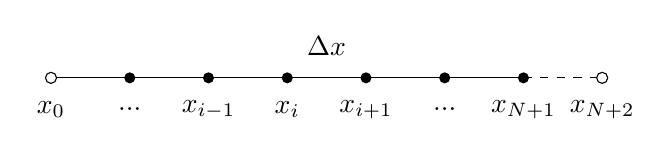
\begin{tikzpicture}
 \draw (0,0) -- (6,0);
 \draw[fill=white](0,0) circle[radius=2pt];
 \fill (1,0) circle[radius=2pt];
 \fill (2,0) circle[radius=2pt];
 \fill (3,0) circle[radius=2pt];
 \fill (4,0) circle[radius=2pt];
 \fill (5,0) circle[radius=2pt];
 \fill (6,0) circle[radius=2pt];
 \node at (0,-0.4) {$x_0$};
 \node at (1,-0.4) {$...$};
 \node at (2,-0.4) {$x_{i-1}$};
 \node at (3,-0.4) {$x_i$};
 \node at (4,-0.4) {$x_{i+1}$};
 \node at (5,-0.4) {$...$};
 \node at (6,-0.4) {$x_{N+1}$};
 \node at (3.5,0.4) {$\Delta x$};
 
 \draw[dashed] (6,0) -- (7,0);
 \draw[fill=white](7,0) circle[radius=2pt];
 \node at (7,-0.4) {$x_{N+2}$};
\end{tikzpicture}
\caption{One-dimensional mesh with constant $\Delta x$.}
\end{figure}
Here, we already took into account that we prescribe Dirichlet boundary conditions at $x_0 = 0$ and homogeneous Neumann boundary conditions at $x_{N+1} = L$. Use central differences for both the first and second derivative.

Derive a semi-discrete matrix formulation of the form,
\begin{align}
\label{MOL}
\dot{\mathbf{u}} = \nu K \mathbf{u} - \mathbf{f}(\mathbf{u}) + \mathbf{r}(\mathbf{u}),
\end{align}
where the vector $\mathbf{r}$ encounters for the boundary conditions, and $\mathbf{f}$ is non-linear. What is the number of unknowns in the vector $\mathbf{u}$?

\textit{Hint: Useful Matlab functions are: } \texttt{linspace, spdiags, u.\^ \! 2}\\
\textit{\phantom{\indent Hint:} Useful Python functions are: } \texttt{numpy.linspace, round, scipy.sparse.spdiags,}\\
\phantom{\indent \textit{Hint: Useful Python functions are: }} \texttt{numpy.array}
\section{Time integration}
\label{ch:euler}
Write a Matlab/Python code to simulate the problem! Use Forward Euler to integrate \eqref{MOL} in time and set the parameters to the values given in Table \ref{params1}. Plot both, the solution $u$ and the car density $\rho$ at every time step. Use a constant time step of $\Delta t = 0.0001$ for now.
\begin{table}[ht]
\centering
 \begin{tabular}{|c|c|c|c|c|}
  \hline
  $\nu$ & $N$ & $L$ & $t_e$ & $\Delta t$\\
  \hline
  $0.5$ & $100$ & $3.0$ & $5.0$ & task \ref{eq:timestep}\\
  \hline
 \end{tabular}
\caption{Parameter configuration.}\label{params1}
\end{table}

\textit{Hint: Useful Matlab functions are: } \texttt{plot, pause(0.05) }\\
\textit{\phantom{\indent Hint:} Useful Python functions are: } \texttt{plt.plot, plt.draw, plt.pause, fig[0].remove}
\section{Stability analysis of the linearized equation}
\label{eq:timestep}
The simulation with the time step of task \ref{ch:euler} is quite slow. We want to investigate how big the time step can be chosen. Therefore, first play with the parameters $\nu$ and $N,L$ in order to get a feeling.

Next, perform a stability analysis based on the linearized equation. Therefore, formulate the discretization stencil at $x=x_i$ in the form,
\begin{align*}
 \dot{u}_i = g_i(\mathbf{u}).
\end{align*}
The Jacobian is then defined as the matrix $[\mathbf{J}]_{i,j} = \frac{\partial g_i}{\partial u_j}$. You can base your stability analysis on the Jacobian evaluated at the initial condition \eqref{eq:init_cond} and the stability region of Euler forward.

\textit{Hint: For the minimum eigenvalue of $J(\mathbf{u}^0)$ you might use Gershgorin's theorem, or review huiswerk \#4.}
\section{Simulation}
Integrate the PDE from $t=0$ to $t_e=5$ using the derived time step $\Delta t$ and $\Delta x$ as defined via Table \ref{params1}. Also increase your derived time step by $1\%$ which shows that the estimation is \textit{sharp}. What happens if we run the simulation for a very long time?

\section{Upwind scheme}
Consider the new initial condition 
\begin{align*}
% \label{eq:init_cond_new}
 u^0(x) = \begin{cases}
           1, &\quad 0 \leq x \leq L/3, \\
           2-(3/L) x, &\quad L/3 \leq x \leq 2L/3,\\
           0, &\quad x \geq 2L/3.
          \end{cases}
\end{align*}
together with (new!) boundary conditions,
\[
 u_l(t) = +1, \quad u_r(t) = 0, \quad t \geq 0.
\]

Again, use Forward Euler for the time integration, and set the parameters to the values given in Table \ref{params2}. Plot both, the solution $u$ and the car density $\rho$ at every time step. Do you observe something strange?

\begin{table}[ht]
\centering
 \begin{tabular}{|c|c|c|c|c|}
  \hline
  $\nu$ & $N$ & $L$ & $t_e$ & $\Delta t$\\
  \hline
  $0.01$ & $100$ & $3.0$ & $5.0$ & $0.003$\\
  \hline
 \end{tabular}
\caption{Parameter configuration.}\label{params2}
\end{table}

In this task, we want to avoid the \textit{strangeness} that appears when using the code developed in task 1-5. Therefore, note that $u>0$ and replace the central discretization for the first derivative in Burgers' equation \eqref{eq:Burgers} by an \textit{upwind scheme}. Use the same parameters as before (as specified Table \ref{params2}).

We want to find out after what time all cars left the road? Therefore, integrate the car density $\rho$ with respect to $x$ at all time steps. Use the Trapezoidal rule and determine when a threshold value of \texttt{0.001} is reached such that \textit{the road is empty}.

% {\color{red}
% \section{Analysis of upwind scheme}
% Consider the inviscid Burgers' equation, that is $\nu = 0$,
% \begin{align}
% \label{eq:inviscid}
%  \frac{\partial u}{\partial t} + \frac{\partial}{\partial x} \left( \frac{1}{2}u^2 \right) = 0.
% \end{align}
% The total variation $TV(u)$ is defined as,
% \begin{align*}
% TV(u^{n}) := \sum_{i} |u_i^{n} - u_{i-1}^{n}|, \quad \text{where } u_i^n = u(x_i,t^n),
% \end{align*}
% and it is known that if $TV(u^{n+1}) \leq TV(u^{n})$ then a monotonic initial condition \eqref{eq:init_cond_new} guarantees a monotonic solution $u^n$ and, hence, no \textit{wiggles} can occur. Show that this holds for an upwind discretization of \eqref{eq:inviscid}.
% 
% \textit{Hint: Structure your proof in the following way:\\
%        \phantom{\indent Hint: }1. Write-down the stencil for $u_i^{n+1}$ using $\mu:=\Delta t/(2 \Delta x)$ and $a^2-b^2 = (a-b)(a+b)$,\\
%        \phantom{\indent Hint: }2. Do the same for $u_{i-1}^{n+1}$,\\
%        \phantom{\indent Hint: }3. Use that $u_i^n \leq \max_i |u_i^n|$, and $\max_i |u_i^n| \frac{\Delta t}{\Delta x} \leq 1$.}
% }

\section*{Contact and further reading}
Many information can be found in:
\begin{itemize}
 \item R. J. Leveque, \textit{Finite Volume Methods for Hyperbolic Problems.} Cambridge Texts in Applied Mathematics, 2002.
\end{itemize}
For questions, you can reach me via \href{mailto:M.M.Baumann@tudelft.nl}{M.M.Baumann@tudelft.nl}.
\end{document}
\end{document}
